\label{sec:appendix}

Example for citing references. References~\cite{dunecdr,montanari_35ton,genie} should be entered in bibliography.tex file under your section.
\begin{verbatim}
Example for citing references. References~\cite{dunecdr,montanari_35ton,genie}.
\end{verbatim}

\vspace{0.5in}


Here is an example of how to insert Fig.~\ref{fig:adc_blockdiagram}. Figures should be saved in ./figures directory.

\begin{figure}[htb]
\centering
%\begin{minipage}[b]{1.0\textwidth}
\begin{center}
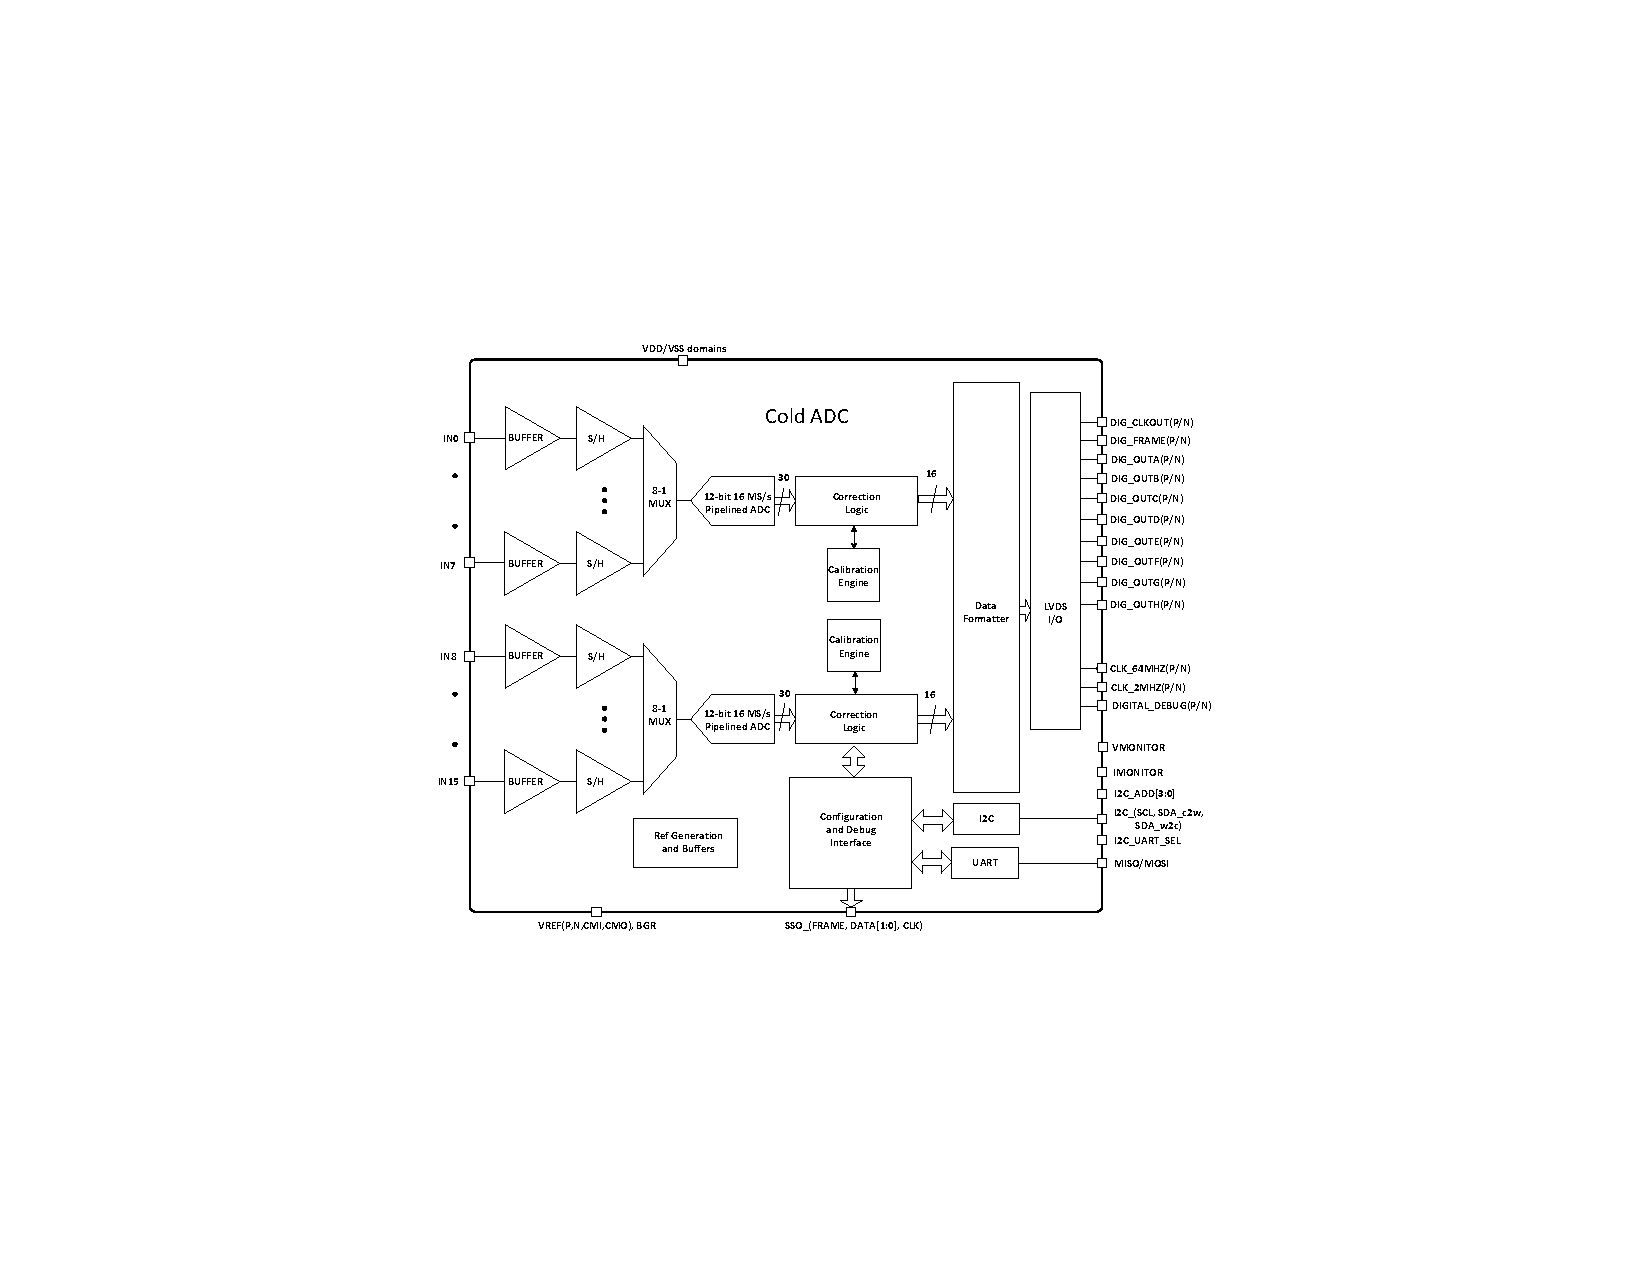
\includegraphics[width=0.7\textwidth]{figures/coldadc_blockdiagram.pdf}
\end{center}
%\end{minipage}
\caption{ColdADC Block Diagram.}
\label{fig:adc_blockdiagram}
\end{figure}

\begin{verbatim}
\begin{figure}[htb]
\centering
\begin{center}
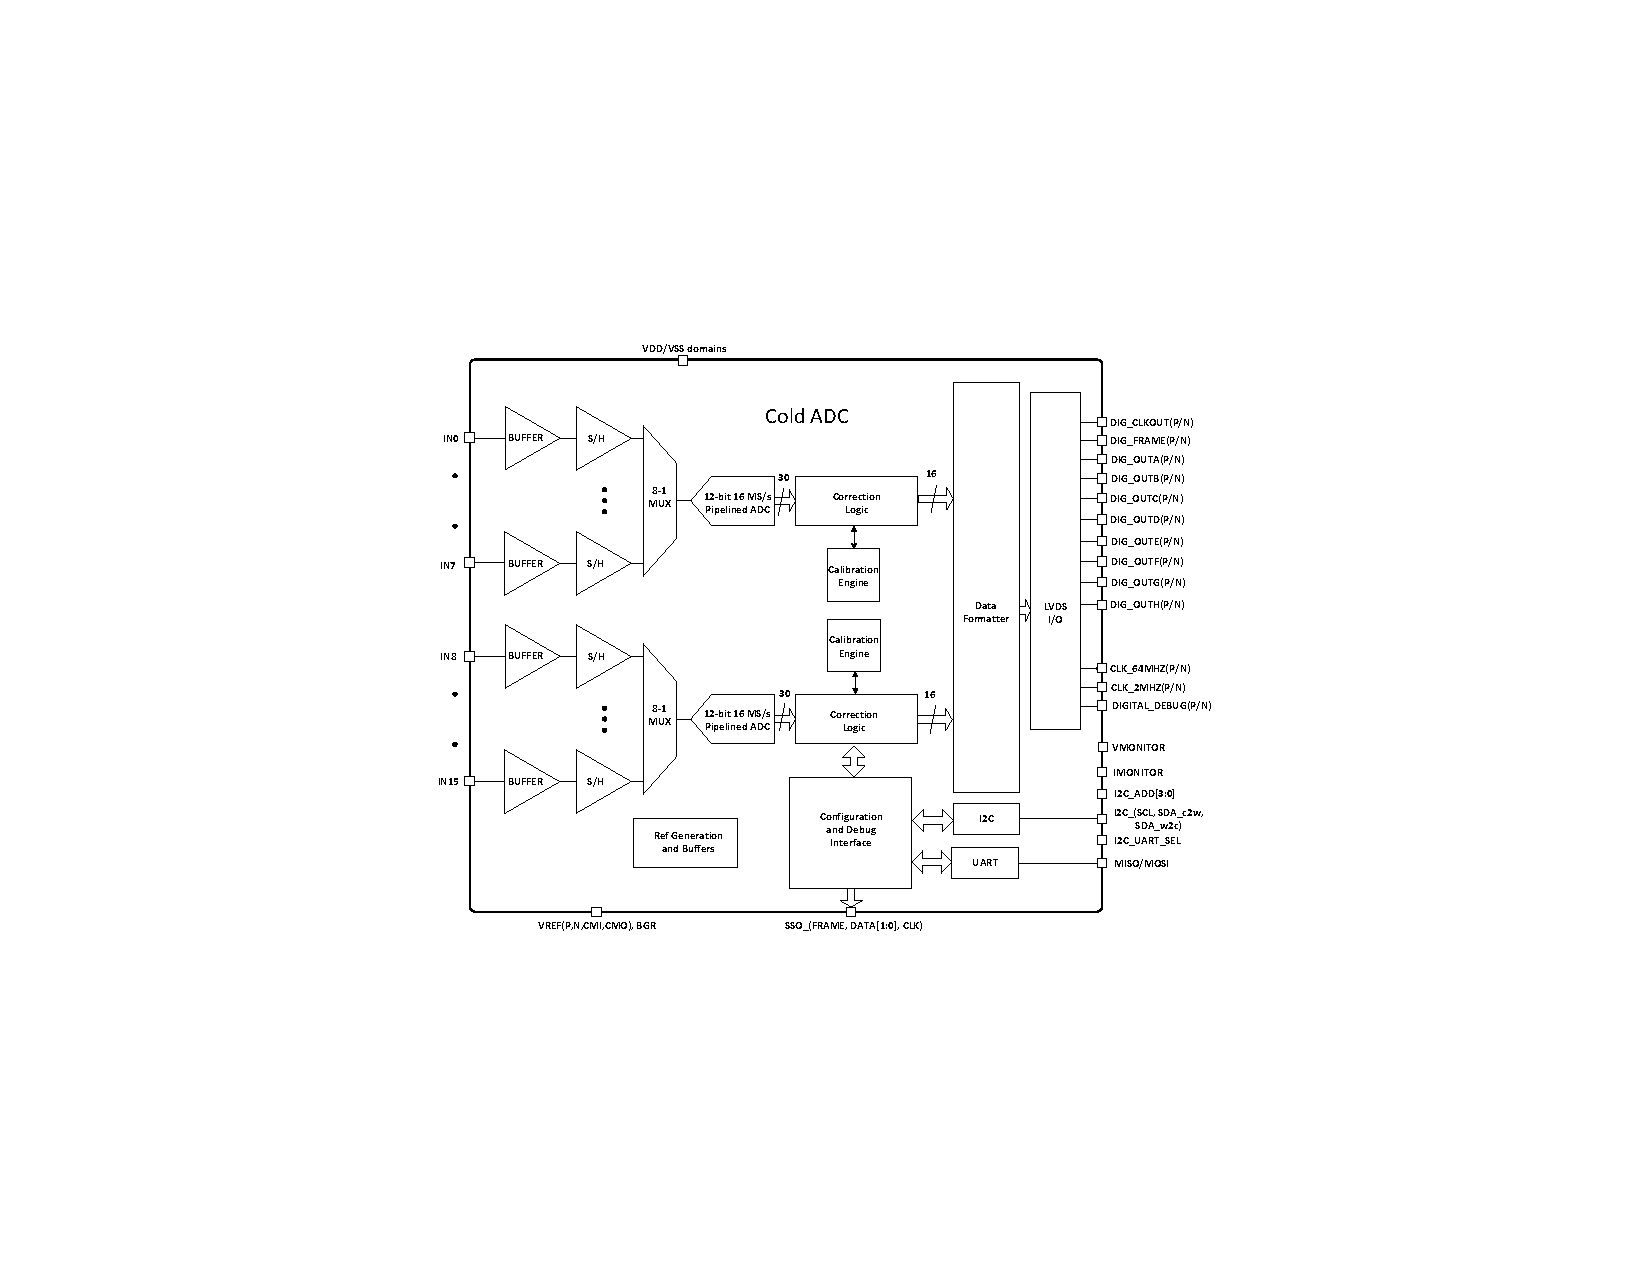
\includegraphics[width=0.7\textwidth]{figures/coldadc_blockdiagram.pdf}
\end{center}
\caption{ColdADC Block Diagram.}
\label{fig:adc_blockdiagram}
\end{figure}
\end{verbatim}


\newpage
Here is an example of how to create Table~\ref{tab:TPC-dim}.

\begin{table}[h]
\centering
\begin{tabular}{|c|c|}
\hline
\textbf{ Component } & dimensions [m]  \\ \hline \hline
APA  (active) &  $2.29 (wide) \times 5.9 (high)$ \\ \hline
APA  (external) &  $2.32 (wide) \times 6.2 (high)$ \\ \hline
TPC (active)       & $7.0 (long) \times 7.2 (wide) \times 5.9 (high)$  \\ \hline
TPC (external)       & $7.3 (long) \times 7.4 (wide) \times 6.2 (high)$  \\ \hline
cryostat (internal) &  $8.9 (long) \times 7.8 (wide) \times 8.1 (high)$  \\ \hline
\end{tabular}
\caption{Dimensions of DUNE-PT.}
\label{tab:TPC-dim}
\end{table}

\begin{verbatim}
\begin{table}[h]
\centering
\begin{tabular}{|c|c|}
\hline
\textbf{ Component } & dimensions [m]  \\ \hline \hline
APA  (active) &  $2.29 (wide) \times 5.9 (high)$ \\ \hline
APA  (external) &  $2.32 (wide) \times 6.2 (high)$ \\ \hline
TPC (active)       & $7.0 (long) \times 7.2 (wide) \times 5.9 (high)$  \\ \hline
TPC (external)       & $7.3 (long) \times 7.4 (wide) \times 6.2 (high)$  \\ \hline
cryostat (internal) &  $8.9 (long) \times 7.8 (wide) \times 8.1 (high)$  \\ \hline
\end{tabular}
\caption{Dimensions of DUNE-PT.}
\label{tab:TPC-dim}
\end{table}

\end{verbatim}

